\documentclass[aspectratio=169]{beamer}
\usepackage{tikz}
\usepackage{graphicx}
\usepackage{listings}
\usepackage{xcolor}
\usepackage{hyperref}
\usepackage[spanish,es-noquoting]{babel}
\usepackage[round]{natbib}

\lstset{
  basicstyle=\ttfamily\small,
  keywordstyle=\color{blue},
  stringstyle=\color{red},
  commentstyle=\color{gray},
  showstringspaces=false
}

% Clean Theme Setup & Optimization
\usetheme{Warsaw}
\usecolortheme{default}
\usefonttheme{serif}

% Remove top headline bar and navigation clutter to maximize slide text space
\setbeamertemplate{headline}{}
\setbeamertemplate{navigation symbols}{}
\setbeamertemplate{frametitle continuation}{}

% Slim, clean footline bar
\setbeamertemplate{footline}{
  \leavevmode%
  \hbox{%
    \begin{beamercolorbox}[wd=.333333\paperwidth,ht=2.25ex,dp=1ex,left]{author in head/foot}%
      \hspace*{2ex}\insertshortauthor
    \end{beamercolorbox}%
    \begin{beamercolorbox}[wd=.333333\paperwidth,ht=2.25ex,dp=1ex,center]{title in head/foot}%
      \insertshorttitle
    \end{beamercolorbox}%
    \begin{beamercolorbox}[wd=.333333\paperwidth,ht=2.25ex,dp=1ex,right]{date in head/foot}%
      \insertframenumber{} / \inserttotalframenumber\hspace*{2ex}
    \end{beamercolorbox}%
  }%
  \vskip0pt%
}

% Font size and list spacing optimizations to prevent text overflow
\setbeamertemplate{itemize/enumerate body begin}{\small}
\setbeamertemplate{itemize/enumerate subbody begin}{\footnotesize}
\setbeamertemplate{itemize/enumerate subsubbody begin}{\scriptsize}

\makeatletter
\g@addto@macro\itemize{%
  \setlength{\itemsep}{2pt}%
  \setlength{\parsep}{1pt}%
  \setlength{\topsep}{2pt}%
  \setlength{\partopsep}{0pt}%
}
\makeatother

\graphicspath{{../}{./}}
\setbeamertemplate{caption}[numbered]

% Title info
\title[ Transformación de la Práctica]{ Transformación de la Práctica Jurídica}
\subtitle{ Lo que la IA sí puede (y no puede) hacer}
\author{Ricardo Reyes-Jimenez}
\institute{Universidad de La Sabana}
\date{\today}


% Background image for title slide
\usebackgroundtemplate{
  \tikz\node[opacity=0.3]{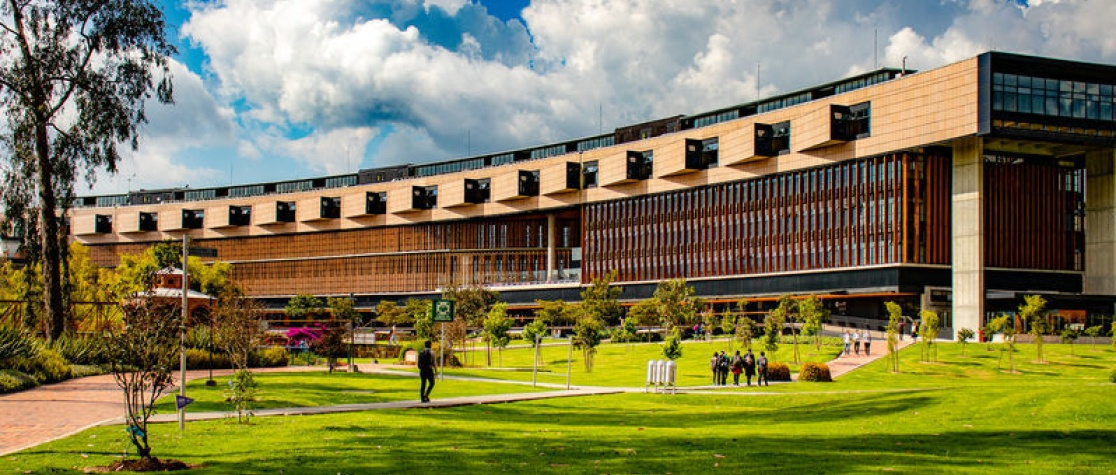
\includegraphics[width=\paperwidth,height=\paperheight]{Images/UniSabana.jpg}};
}


\begin{document}

% Title slide
\begin{frame}
  \titlepage
\end{frame}

% Reset background for normal slides
\usebackgroundtemplate{}


\begin{frame}[allowframebreaks,fragile]{Introducción al Módulo 1.2}


Este módulo profundiza en cómo la Inteligencia Artificial Generativa está cambiando la práctica jurídica diaria, estableciendo qué tareas pueden delegarse de manera segura y cuáles son los límites técnicos actuales.

\end{frame}

\begin{frame}[allowframebreaks,fragile]{Resolviendo Dudas del Público (Q\&A)}


Antes de profundizar, resolvamos tres inquietudes clave que surgieron en la primera sesión:

\textbf{1. ¿Cómo puedo estar seguro de no infringir derechos de autor de terceros?}
\begin{itemize}
  \item \textbf{La Regla de Oro:} Evite pedirle a la IA que genere contenido basándose en obras protegidas específicas de terceros. Utilice la IA para analizar o redactar a partir de \textit{sus propias} plantillas (o las de la firma) \cite{dnda2023}.
  \item \textbf{Protección Enterprise:} Herramientas comerciales (como Copilot o Claude Enterprise) incluyen cláusulas de \textit{Indemnización por Copyright}, protegiendo al usuario si el modelo genera contenido infractor de manera inadvertida.
\end{itemize}
\end{frame}

\begin{frame}[allowframebreaks,fragile]{Resolviendo Dudas del Público (Q\&A) - Parte 2}


\textbf{2. ¿Cómo vencer la resistencia por el impacto ambiental de la IA?}
\begin{itemize}
  \item \textbf{El Problema:} Entrenar y consultar modelos gigantes consume mucha energía y agua.
  \item \textbf{Mitigación (Uso Eficiente):} Use el modelo ``adecuado'' para la tarea. No use el modelo más potente y pesado (ej. GPT-4o o Claude Opus) para resumir un correo simple; use modelos ligeros, rápidos y de bajo consumo (GPT-4o-mini o Claude Haiku). La eficiencia computacional reduce la huella de carbono.
\end{itemize}
\textbf{3. ¿Cómo hago para incluir las referencias o citas legales?}
\begin{itemize}
  \item \textbf{El Peligro:} Los LLMs abiertos (como ChatGPT) inventan (alucinan) sentencias y leyes.
  \item \textbf{La Solución (Grounding / RAG):} Debe usar herramientas que ``anclen'' la respuesta a una base de datos legal verificada (Lexis+ AI, vLex) o subir sus propios PDFs a herramientas como \textbf{NotebookLM}, donde la IA está forzada a incluir el número de página y la cita exacta del documento subido.
\end{itemize}
\end{frame}

\begin{frame}[allowframebreaks,fragile]{Ética y Uso Responsable (Gemini)}


El análisis de documentos legales con IA exige un estándar ético riguroso:

\begin{itemize}
  \item \textbf{Privilegio Abogado-Cliente:} El abogado sigue siendo el garante del secreto profesional.
  \item \textbf{Sesgos y Equidad:} La IA puede heredar sesgos de sus datos de entrenamiento.
  \item \textbf{Responsabilidad de Uso (Gemini):} Se debe usar como asistente y no como tomador de decisiones. El output debe ser siempre revisado por un humano.
\end{itemize}
\end{frame}

\begin{frame}[allowframebreaks,fragile]{Privacidad: ¿A dónde va la información?}




El uso de modelos gratuitos (como ChatGPT o Gemini básico) conlleva riesgos de privacidad:

\begin{itemize}
  \item \textbf{Modelos Gratuitos:} Por defecto, los datos ingresados (prompts) \textbf{pueden ser utilizados} para entrenar futuras versiones del modelo \cite{geminiprivacy}.
  \item \textbf{Pérdida de Confidencialidad:} Introducir datos reales de un cliente en estas versiones viola los deberes éticos.
  \item \textbf{Solución:} Utilizar versiones \textbf{Enterprise/Corporativas}, modelos locales, o desactivar explícitamente el uso de datos para entrenamiento.
\end{itemize}
\end{frame}

\begin{frame}[allowframebreaks,fragile]{Debate Plenario: El Caso del Contrato Subido a la Nube}


\textbf{Escenario:}
Un asociado junior revisa un contrato de compraventa de acciones confidencial. Para agilizar, copia todo el texto (con nombres reales, precios y datos personales) en el ChatGPT gratuito pidiendo un resumen de riesgos.

\textbf{Preguntas de Discusión:}
\begin{itemize}
  \item ¿Hubo transmisión internacional de datos no autorizada (Ley 1581)?
  \item ¿Se violó el secreto profesional o la confidencialidad?
  \item ¿Qué pasa si la plataforma es hackeada o usa esos datos para generar respuestas a terceros?
  \item ¿Cómo debió proceder el asociado de forma segura?
\end{itemize}
\end{frame}

\begin{frame}[allowframebreaks,fragile]{El Nuevo Modelo de Negocio Legal}


\begin{itemize}
  \item \textbf{El fin del modelo tradicional:} La transición de las horas facturables (billable hours) a los honorarios por valor (value-based pricing).
  \item \textbf{La paradoja de la eficiencia:} ¿Cómo facturar si la IA reduce un análisis de \textit{due diligence} de 10 horas a 5 minutos?
  \item \textbf{Ventaja competitiva:} ``La IA no reemplazará a los abogados, pero los abogados que usan IA reemplazarán a los que no la usan''. La tecnología permite escalar el volumen de casos sin aumentar la plantilla linealmente.
\end{itemize}
\end{frame}

\begin{frame}[allowframebreaks,fragile]{Ejemplo: Del ``Billable Hour'' al ``Value-Based''}


\textbf{¿Qué pasa cuando somos más rápidos?}
\begin{itemize}
  \item \textbf{El Modelo Antiguo:} La firma A tarda 10 horas en revisar contratos a $200/h = $2,000.
  \item \textbf{El Modelo IA:} La firma B usa IA, tarda 2 horas y cobra por ``paquete de revisión'' a $1,500 fijos.
  \item \textbf{El Resultado:} El cliente ahorra $500 y obtiene el trabajo en menos tiempo. La firma B aumentó su rentabilidad por hora drásticamente y puede tomar más clientes. ¡La eficiencia no penaliza los ingresos si cambia el modelo de cobro!
\end{itemize}
\end{frame}

\begin{frame}[allowframebreaks,fragile]{Lo que la IA SÍ puede (y NO puede) hacer}


\begin{table}
\resizebox{\textwidth}{!}{
\begin{tabular}{|l | l | l|}
\hline
\textbf{Tarea Jurídica} & \textbf{Nivel de Riesgo} & \textbf{Recomendación} \\ \hline
Redacción de correos y memos simples & Bajo & Uso rutinario con supervisión básica \\ \hline
Búsqueda de jurisprudencia en bases abiertas & Alto & NO RECOMENDADO (Riesgo de alucinación) \\ \hline
Resumen de expedientes largos & Medio & Ideal para IA, validando contra el PDF original \\ \hline
Análisis predictivo de sentencias & Alto & Requiere herramientas especializadas (ej. Lexis+ AI) \\ \hline
\end{tabular}
}
\end{table}
\end{frame}

\begin{frame}[allowframebreaks,fragile]{Matriz de Impacto en Tareas Diarias}


\begin{itemize}
  \item \textbf{Drafting (Redacción):} \textit{Alto impacto}. Ideal para borradores de contratos estándar, \textit{term sheets} y memos iniciales.
  \item \textbf{Review (Revisión):} \textit{Impacto medio-alto}. Excelente para extracción de cláusulas clave, metadatos y análisis \textit{red-flagging}.
  \item \textbf{Research (Investigación):} \textit{Riesgoso sin RAG}. Peligro crítico de alucinaciones si se usan herramientas abiertas (como ChatGPT) para buscar jurisprudencia.
  \item \textbf{Estrategia Legal y Negociación:} \textit{Impacto bajo}. La IA es un copiloto, pero no reemplaza la empatía, el \textit{leverage} comercial ni la táctica judicial humana.
\end{itemize}
\end{frame}

\begin{frame}[allowframebreaks,fragile]{Ejercicio Flash 1 (2 min): ¿IA, Humano o Híbrido?}


\textbf{Dinámica:} Levanten la mano según quién debe hacer la tarea:
\begin{itemize}
  \item Buscar jurisprudencia para un caso de casación complejo. \textit{(Humano / Herramienta RAG)}
  \item Redactar el primer borrador de un NDA estándar. \textit{(IA)}
  \item Convencer a un cliente de aceptar un acuerdo extrajudicial. \textit{(Humano)}
  \item Revisar si 500 contratos tienen cláusula de cambio de control. \textit{(IA)}
\end{itemize}
\textbf{Lección:} La IA es excelente para volumen y borradores, pero ineficaz para estrategia y empatía pura.

\end{frame}

\begin{frame}[allowframebreaks,fragile]{El Síndrome de la Hoja en Blanco}


\textbf{Cómo la IA cambia el inicio del trabajo:}
\begin{itemize}
  \item \textbf{El problema histórico:} El mayor esfuerzo en la redacción legal es pasar del documento en blanco al primer borrador.
  \item \textbf{La solución GenAI:} La IA actúa como un ``rompehielos''. Produce un borrador de calidad media (un 6/10) en segundos.
  \item \textbf{El nuevo rol del abogado:} Pasamos de ser \textit{redactores} a ser \textit{editores} (llevar ese borrador del 6/10 al 10/10).
\end{itemize}
\end{frame}

\begin{frame}[allowframebreaks,fragile]{Ejercicio Flash 2 (3 min): Red-Flagging Contractual}


\textbf{Contexto:} Lean esta cláusula: \textit{``El proveedor realizará los mejores esfuerzos comerciales para entregar a tiempo.''}
\textbf{Dinámica:}
\begin{itemize}
  \item ¿Qué riesgo ven como abogados? (Tienen 1 minuto).
  \item \textit{Ahora veamos qué dice la IA:} ``La expresión 'mejores esfuerzos comerciales' es subjetiva y no constituye una obligación de resultado, dificultando la ejecución por retrasos.''
\end{itemize}
\textbf{Lección:} La IA no reemplaza su conocimiento, pero asegura que no pasen por alto riesgos por fatiga visual.

\end{frame}

\begin{frame}[allowframebreaks,fragile]{Casos de Uso Reales en la Práctica}


\begin{itemize}
  \item \textbf{Investigación y Análisis Legal:} Utilizar la IA para encontrar patrones en grandes volúmenes de documentos, no para buscar la ``verdad'' legal.
  \item \textbf{Revisión de Contratos:} Identificar cláusulas faltantes o riesgosas (Ej. cláusulas de indemnidad asimétricas).
  \item \textbf{Orientación a Clientes:} Redactar respuestas iniciales en lenguaje claro y accesible.
  \item \textbf{Gestión Documental:} Extracción de metadatos (fechas, partes, montos) de expedientes masivos.
\end{itemize}
\end{frame}

\begin{frame}[allowframebreaks,fragile]{El Peligro de la Confianza Ciega (Mata v. Avianca)}


\textbf{El puente entre el potencial y el riesgo:}

En 2023, abogados en EE. UU. usaron ChatGPT para investigar jurisprudencia y presentaron un escrito con casos que la IA \textbf{inventó (alucinó)} \cite{matavavianca}.

\begin{itemize}
  \item Fueron sancionados por el juez.
  \item Demostró que delegar la investigación sin verificación es negligencia profesional grave.
\end{itemize}
\end{frame}

\begin{frame}[allowframebreaks,fragile]{Anatomía de una Alucinación: ¿Por qué inventa?}


\textbf{¿Por qué una máquina tan ``inteligente'' miente?}
\begin{itemize}
  \item \textbf{No es un buscador:} Los LLMs no buscan en una base de datos. Son calculadoras de probabilidades de palabras \cite{openai2023}.
  \item \textbf{El ``Autocompletar'' con esteroides:} Si le piden una sentencia que no existe, el modelo calculará las palabras que estadísticamente \textit{deberían} estar ahí (nombres, fechas) y generará un texto que \textit{suena} real.
  \item \textbf{Solución:} ¡Nunca le pida hechos a un modelo abierto sin darle el contexto documental!
\end{itemize}
\end{frame}

\begin{frame}[allowframebreaks,fragile]{El Sesgo de Automatización}


\textbf{El riesgo psicológico oculto de la IA:}
\begin{itemize}
  \item \textbf{Definición:} La tendencia humana a confiar ciegamente en sistemas automatizados, incluso ignorando nuestra propia intuición.
  \item \textbf{El Peligro Legal:} Cuando la IA genera un documento con lenguaje formal e impecable, el cerebro asume que es correcto y disminuye su nivel de alerta.
  \item \textbf{Regla de oro:} Lea el documento generado por la IA con \textit{el doble} de escepticismo con el que leería el trabajo de un practicante novato.
\end{itemize}
\end{frame}

\begin{frame}[allowframebreaks,fragile]{Human-in-the-Loop (HITL) como Estándar}


\begin{itemize}
  \item \textbf{La IA propone, el Humano dispone.}
  \item Ningún proceso legal crítico debe ser automatizado de extremo a extremo sin una revisión humana (HITL).
  \item \textbf{Beneficio Dual:} Reduce el riesgo de mala praxis a casi cero, mientras mantiene un ahorro de tiempo sustancial en la fase de generación.
\end{itemize}
\end{frame}

\begin{frame}[allowframebreaks,fragile]{Límites Críticos de la IA Generativa}


\begin{itemize}
  \item \textbf{Falta de Actualización:} Los modelos fundacionales tienen una fecha de corte de conocimiento. No conocen la ley aprobada ayer.
  \item \textbf{Falta de Hechos Específicos:} La IA no conoce el contexto único de su cliente a menos que usted se lo proporcione.
  \item \textbf{Alucinaciones:} La tendencia de la IA a inventar respuestas plausibles pero falsas cuando no tiene información suficiente.
\end{itemize}
\end{frame}

\begin{frame}[allowframebreaks,fragile]{Protocolo de Verificación Legal}


\begin{itemize}
  \item \textbf{Grounding (Anclaje):} Proporcionar a la IA los documentos fuente sobre los cuales debe basar su respuesta.
  \item \textbf{Prompts Restrictivos:} Instruir explícitamente a la IA: ``Responde ÚNICAMENTE basado en los documentos adjuntos''.
  \item \textbf{Verificación Humana:} El abogado siempre debe revisar el documento final. La responsabilidad legal recae en el humano.
\end{itemize}
\end{frame}

\begin{frame}[allowframebreaks,fragile]{Ejercicio Flash 3 (3 min): Mejorando el Prompt}


\textbf{Dinámica:} Tienen 1 minuto para transformar este prompt inútil en uno profesional:
\begin{itemize}
  \item \textbf{Prompt Original:} \textit{``Resume este documento.''}
  \item \textbf{Construyendo el Prompt (Público):} ¿Qué le falta? (Rol, Formato, Restricciones) \cite{murray2024}.
  \item \textbf{El Prompt Ideal (Resultado):} \textit{``Actúa como abogado senior de M\&A. Resume el contrato adjunto enfocándote SOLO en las cláusulas de terminación anticipada. Entrégalos en una tabla con la sección y la explicación. Si no hay cláusula, di 'No Encontrada'. No inventes información.''}
\end{itemize}
\end{frame}

\begin{frame}[allowframebreaks,fragile]{Flujo de Verificación (Ejemplo Práctico)}


\begin{center}
\resizebox{0.9\textwidth}{!}{
\begin{tikzpicture}[node distance=3cm, auto, thick,
box/.style={rectangle, draw=blue!80, fill=blue!10, very thick, text width=3.5cm, align=center, rounded corners, minimum height=1.5cm},
arrow/.style={->, >=stealth, very thick, blue!80}]
\node[box] (n1) {1. Subir PDF del Contrato (Grounding)};
\node[box, right of=n1, xshift=1.5cm] (n2) {2. Prompt restrictivo para extracción};
\node[box, right of=n2, xshift=1.5cm] (n3) {3. Verificar respuesta contra original};
\draw[arrow] (n1) -- (n2);
\draw[arrow] (n2) -- (n3);
\end{tikzpicture}
}
\end{center}

\end{frame}

\begin{frame}[allowframebreaks,fragile]{Deber de Competencia Tecnológica}


\begin{itemize}
  \item \textbf{Actualización del ``Deber de Competencia'':} En múltiples jurisdicciones (ej. \textit{American Bar Association, Rule 1.1}), el deber del abogado ya incluye entender los beneficios y riesgos de la tecnología relevante.
  \item \textbf{Impacto en el Cliente:} Cobrar excesivamente por tareas manuales que una herramienta tecnológica podría hacer en minutos podría considerarse un cobro irrazonable en el futuro cercano.
  \item \textbf{El Abogado Biónico:} La adopción de IA Generativa dejó de ser un ``lujo'' de innovación para convertirse en una necesidad de diligencia profesional.
\end{itemize}
\end{frame}

\begin{frame}[allowframebreaks,fragile]{Ejercicio Práctico: Grounding con NotebookLM}


\textbf{Herramienta:} Gemini Notebook \cite{notebooklm2024}

\textbf{Objetivo:} Interactuar con un expediente masivo sin riesgo de alucinaciones.

\begin{itemize}
  \item Subir la sentencia o expediente en PDF.
  \item Generar una guía de estudio automática.
  \item Hacer preguntas específicas al documento.
  \item Verificar las citas (Gemini Notebook muestra de qué página extrajo la información).
\end{itemize}
\end{frame}

\begin{frame}[allowframebreaks,fragile]{¡Sigamos en Contacto!}


La Inteligencia Artificial avanza todos los días. ¡No duden en escribirme para compartir ideas, resolver dudas o seguir conversando sobre cómo la IA puede transformar su práctica jurídica!

\begin{itemize}
  \item \textbf{WhatsApp:} (57) 3012726157
  \item \textbf{Email:} \href{mailto:rareyesj@gmail.com}{rareyesj@gmail.com}
\end{itemize}
\textbf{¡Muchas gracias por su participación!}


\end{frame}



\begin{frame}[allowframebreaks]{References}
  \bibliographystyle{apalike}
  \bibliography{references}
\end{frame}


\end{document}